\documentclass[11pt]{article}
\usepackage[margin=1in]{geometry}
\usepackage{graphicx}
\usepackage{booktabs}
\usepackage{amsmath}
\usepackage{hyperref}
\usepackage[T1]{fontenc}
\graphicspath{{../../results/gap_guided_inference/}}
\title{Gap-guided LLM inference: a routing contract}
\author{CFPerm prototype}
\date{}
\begin{document}
\maketitle
\noindent Stage-1 modality-gap scores are a frozen routing contract for a model that
can inspect only $k$ channels (tools, RAG indices, prompt sections).
They do not retrain the LLM. $\hat e$ is $P(W{=}1\mid X)$, not $P(Y\mid X)$.

\section{Online packet}
For each query $x$, blend $r_m(x)=\lambda\pi_m+(1-\lambda)s_m(x)$ with
$s_m(x)=\lvert\hat e(x)-\hat e(x_{-m})\rvert/\sum_{m'}\lvert\cdot\rvert$.
Gates (defaults): $\tau_{\mathrm{hi}}=0.42$ enables one tool;
cost budget and $k_{\max}$ pack the rest by $r_m/\mathrm{cost}$;
entropy $\ge 0.92\log M$ abstains and asks for the top channel.
The chat schema never includes $W$ or the TMLE $H_m$ (those use the batch label).
$H_m$ stays in outcome training.

Copy-paste artifacts live in \texttt{gap\_guided\_inference.py}:
\texttt{render\_system\_prompt}, \texttt{openai\_tool\_schema}, \texttt{critic\_check}.

\section{Budgeted-block stand-in (no vendor LLM)}
A block RF that only reads $B_m$ is the same decision as packing one modality
into the context window. The ceiling is the oracle GT block.
Wide text plus a concentrated valence shift is the regime where raw VIMP
overweights width and $\pi$ should route to valence.
Shuffle-valence is the negative control: hit rate on that name must collapse.
The inject row is the shipping check: VIMP selects the wide text block (hit 0),
$\pi$ selects valence (hit 1), and the routed expert's AUC matches the oracle.

\begin{table}[h]
\centering
\small
\caption{Held-out domain AUC of a one-block expert (mean of 3 seeds).}
\begin{tabular}{lccccc}
\toprule
Setting & oracle & blend $r$ & $\pi$ & VIMP & random \\
\midrule
synthetic GT=valence & 0.959 & 0.957 & 0.959 & 0.959 & 0.642 \\
inject valence & 0.747 & 0.745 & 0.747 & 0.600 & 0.583 \\
shuffle valence (neg.) & 0.505 & 0.481 & 0.474 & 0.470 & 0.516 \\
\bottomrule
\end{tabular}
\end{table}

\begin{table}[h]
\centering
\small
\caption{$P(\textrm{selected block}=\textrm{GT})$ under a one-tool budget.}
\begin{tabular}{lccccc}
\toprule
Setting & blend $r$ & $\pi$ & instance $s$ & VIMP & random \\
\midrule
synthetic GT=valence & 0.980 & 1.000 & 0.749 & 1.000 & 0.231 \\
inject valence & 0.824 & 1.000 & 0.465 & 0.000 & 0.245 \\
shuffle valence (neg.) & 0.128 & 0.333 & 0.191 & 0.000 & 0.256 \\
\bottomrule
\end{tabular}
\end{table}

\begin{figure}[h]
\centering
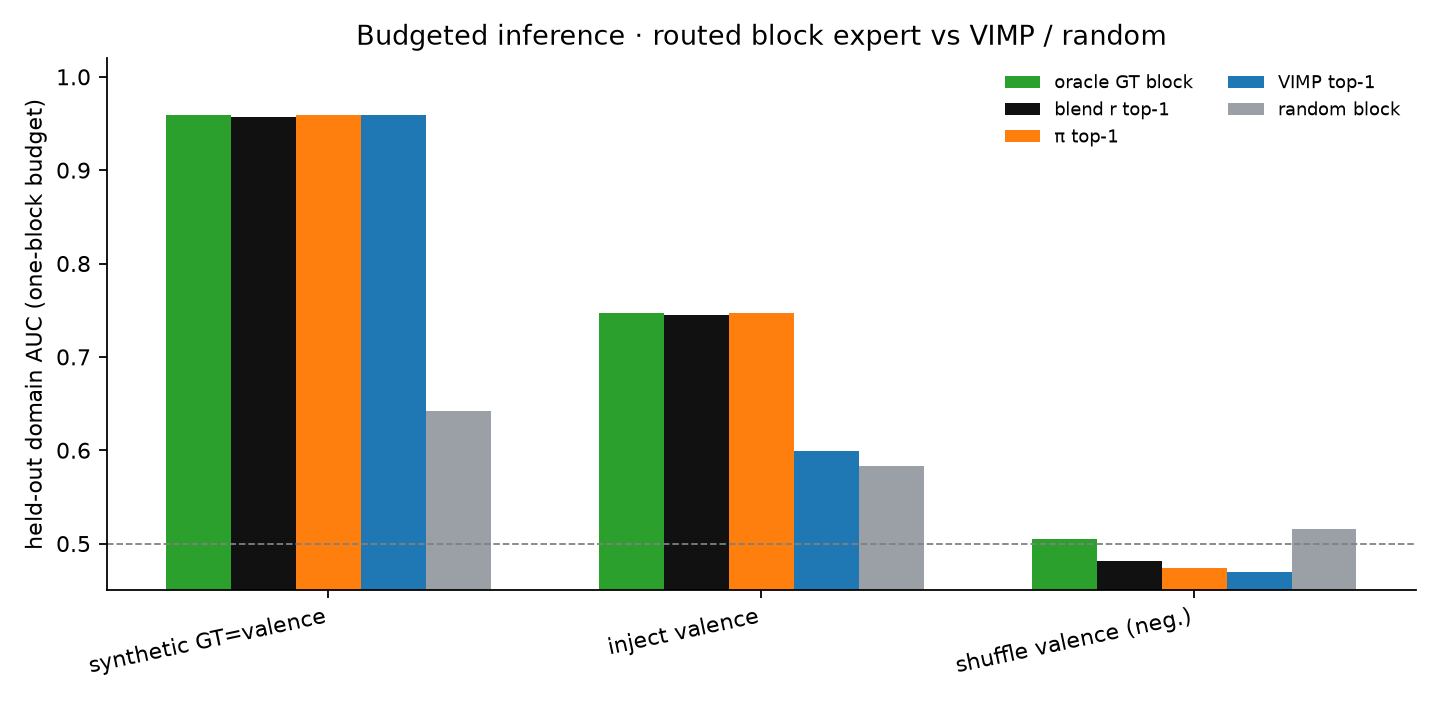
\includegraphics[width=\textwidth]{budgeted_auc.png}
\caption{Held-out domain AUC of the routed one-block expert.}
\end{figure}

\begin{figure}[h]
\centering
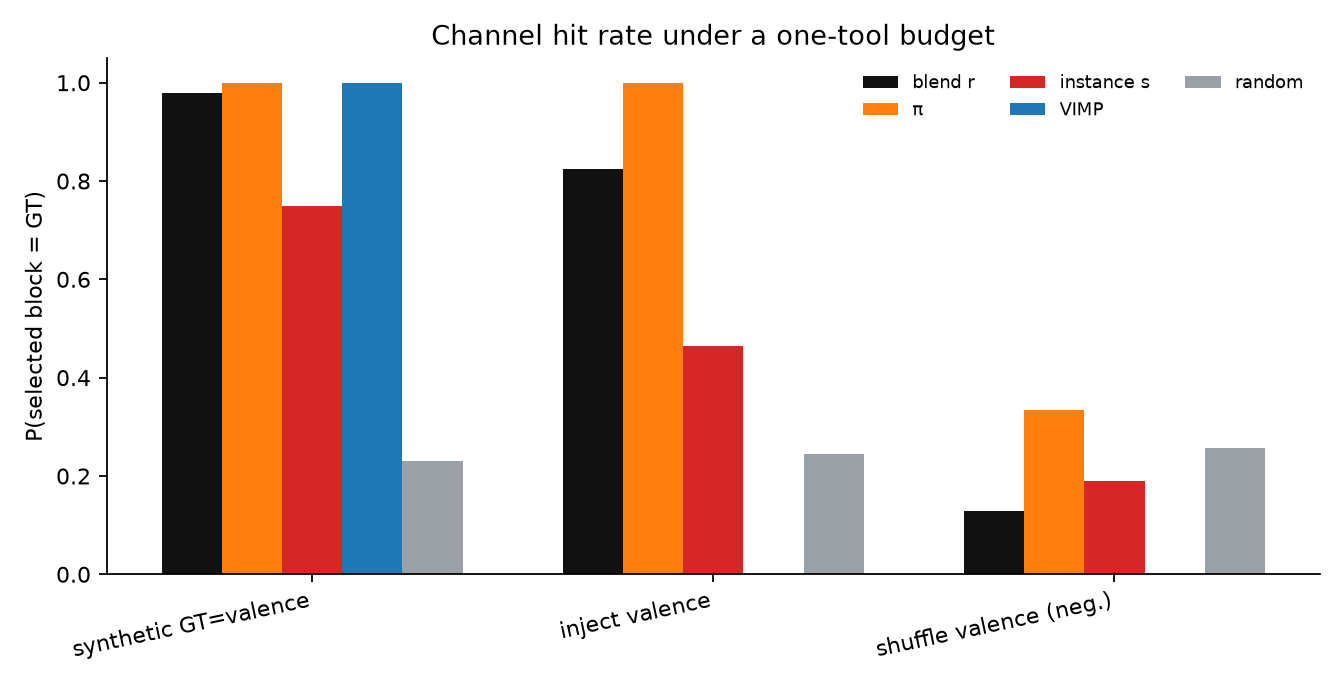
\includegraphics[width=\textwidth]{gt_hit_rate.png}
\caption{$P(\textrm{selected block}=\textrm{GT})$ under a one-tool budget.}
\end{figure}

Diffuse observational shifts are not a routing win; the same honesty as Stage-2.
Ship the gate when the channel is concentrated; keep $\pi$ as a prior when $H(r)$ is high.

\end{document}
